\section{Monday for MAT4002}\index{Monday_lecture}
\paragraph{Reviewing}
Consider the group with presentation $\langle S\mid R(S)\rangle$.
\begin{enumerate}
\item
The elements in $S$ are generators that have studied in abstract algebra
\item
The ``relations'' of this group are given by the equalities on hte right-hand side, e.g.,
the dihedral group is defined as
\[
\langle a,b\mid a^n=e,b^2=e,bab=a^{-1}\rangle
\]
Sometimes we also simplify the equality $\times = e$ as $\times$, e.g., the dihedral group can be re-written as
\[
\langle a,b\mid a^n,b^2,bab=a^{-1}\rangle
\]
\end{enumerate}

\begin{example}
Consider 
\[
G=<a,b\mid a^2,b^2,abab^{-1}a^{-1}b^{-1}>:=
<a,b\mid a^2,b^2,aba=bab>
=
\{
e,a,b,ab,ba,aba
\}
\]
It's isomorphic to $S^3$, and the shape of $S^3$ is illustrated in Fig.(\ref{Fig:11:1})
\begin{figure}[H]
	\centering{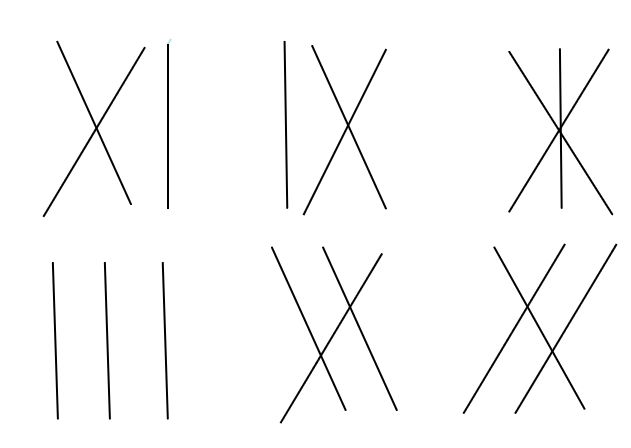
\includegraphics[width=6cm]{week11/S3group.png}}
	\caption{Illustration of group $S^3$}
	\label{Fig:11:1}
\end{figure}

More precisely, the isomorphism is given by:
\[
\begin{array}{ll}
\phi:&S_3\to G\\
\text{with}&X\mid\mapsto a,\quad
\mid X\mapsto b
\end{array}
\]
\end{example}





\begin{example}
Consider $G_2=<a,b\mid ab=ba>$ and any word, which can be expressed as $\cdots a^sb^ta^ub^v\cdots$
\begin{itemize}
\item
If $s\in\mathbb{N}$, we write $a^s:=\underbrace{a\cdots a}_{s\text{ times}}$
\item
If $s\in-\mathbb{N}$, we write $a^s:=\underbrace{(a^{-1})\cdots (a^{-1})}_{-s\text{ times}}$
\item
For the word with the form $a\cdots b\cdots b a\cdots a$, we can always push $a$ into the leftmost using the relation $ab=ba$
\item
For the word with the form $a\cdots a b\cdots ba^{-1}$, we can always push $a^{-1}$ into the leftmost using the relation $ba^{-1}=a^{-1}b$.
\end{itemize}
Therefore, all elements in $G_2$ are of the form $a^pb^q,p,q\in\mathbb{Z}$, and we have the relation
\[(a^{p_1}b^{q_1})(a^{p_2}b^{q_2})=a^{p_1+p_2}b^{q_1+q_2}.\]
Therefore, $G_2\cong \mathbb{Z}\times\mathbb{Z}$, where the isomorphism is given by:
\[
\begin{array}{ll}
\phi:&\mathbb{Z}\times\mathbb{Z}\to G_2\\
\text{with}&(p,q)\mapsto a^pb^q
\end{array}
\]
\end{example}

\begin{example}
\[
G_3=\langle a\mid a^5\rangle=\{1,a,a^2,\dots,a^4\}
\]
It's clear that $G_3\cong \mathbb{Z}/5\mathbb{Z}$, where the isomorphism is given by:
\[
\begin{array}{ll}
\phi:&\mathbb{Z}/5\mathbb{Z}\to G_3\\
\text{with}&m+5\mathbb{Z}\mapsto a^m
\end{array}
\]
\end{example}

\subsection{Cayley Graph for finitely presented groups}
Graphs have strong connection with groups. Here we introduce a way of building graphs using groups, and the graphs are known as Cayley graphs.
They describe many properties of the group in a topological way.
\begin{definition}[Oriented Graph]
An oriented graph $T$ is specified by
\begin{enumerate}
\item
A countable or finite set $V$, known as vertices
\item
A countable or finite set $E$, known as edges
\item
A function $\delta:E\to V\times V$ given by
\[
\delta(e) = (\ell(e),\tau(e))
\]
where $\ell(e)$ denotes the initial vertex and $\tau(e)$ denotes the terminal vertex.
\end{enumerate}
\end{definition}
For example, let 
\begin{itemize}
\item
$V=\{a,b,c\}$
\item
$E=\{e_1,e_2,e_3,e_4\}$
\item
$\delta(e_1)=(a,a),
\delta(e_2)=(b,c),
\delta(e_3)=(a,c),
\delta(e_4)=(b,c)$
\end{itemize}
\begin{figure}[H]
	\centering{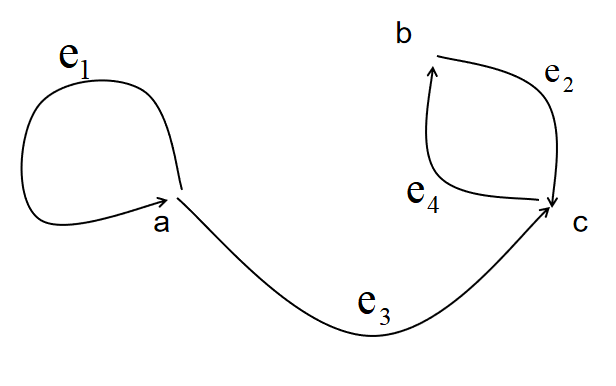
\includegraphics[width=6cm]{week11/cayley1.png}}
	\caption{Illustration of example oriented graph}
	\label{Fig:11:2}
\end{figure}
The resulted graph is plotted in Fig.(\ref{Fig:11:2})


\begin{definition}[Cayley graph]
Let $G=\langle S\mid R(S)\rangle$ with $|S|<\infty$.
The \emph{Cayley graph} associated to $G$ is an oriented graph with
\begin{enumerate}
\item
The vertex set $G$
\item
The edge set $E:=G\times S$
\item
The function $\ell:E\to V\times V$ is given by:
\[
\begin{array}{ll}
\ell:&G\times S\to G\times G\\
\text{with}&(g,s)\mapsto(g,g\cdot s)
\end{array}
\]
\end{enumerate}
In particular, we link two elements in $G$ if they differ by a generator rightside.
\end{definition}
\begin{example}
\begin{enumerate}
\item
The Cayley graph for $G=\langle a\rangle$ $(\cong\mathbb{Z})$ is shown in Fig.(\ref{Fig:11:3}):
\begin{figure}[H]
	\centering{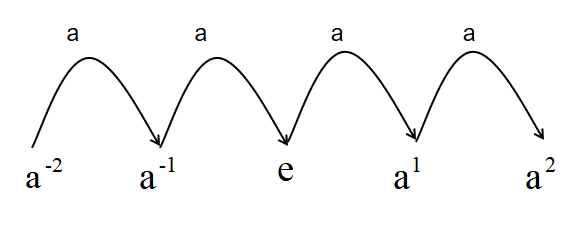
\includegraphics[width=0.7\textwidth]{week11/cayley2.png}}
	\caption{Illustration of Cayley Graph $\langle a\rangle$}
	\label{Fig:11:3}
\end{figure}
\item
The Cayley graph for $G=\langle a\mid a^3\rangle$ is shown in Fig.(\ref{Fig:11:5}):
\begin{figure}[H]
	\centering{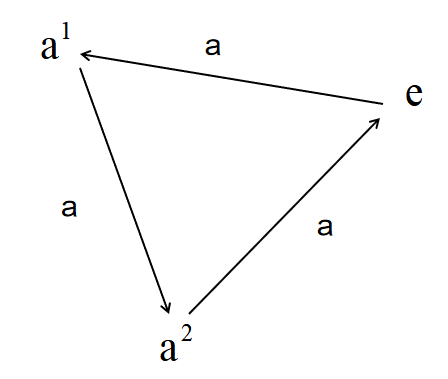
\includegraphics[width=0.4\textwidth]{week11/cayley3.png}}
	\caption{Illustration of Cayley Graph $\langle a\mid a^3\rangle$}
	\label{Fig:11:5}
\end{figure}

\item
The Cayley graph for $G=\langle a,b\mid a^2,b^2,aba=bab\rangle$ is shown in Fig.(\ref{Fig:11:6}):
\begin{figure}[H]
	\centering{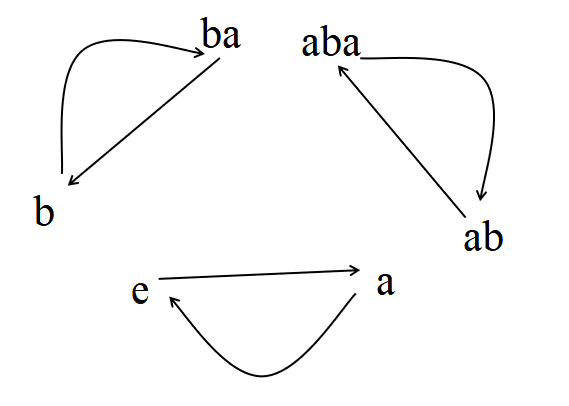
\includegraphics[width=0.3\textwidth]{week11/cayley4.png}}
	\caption{Illustration of Cayley Graph $\langle a,b\mid a^2,b^2,aba=bab\rangle$}
	\label{Fig:11:6}
\end{figure}
\item
The Cayley graph for $G=\langle a,b\mid ab=ba\rangle$ is shown in Fig.(\ref{Fig:11:7:a}):
\begin{figure}[H]
	\centering{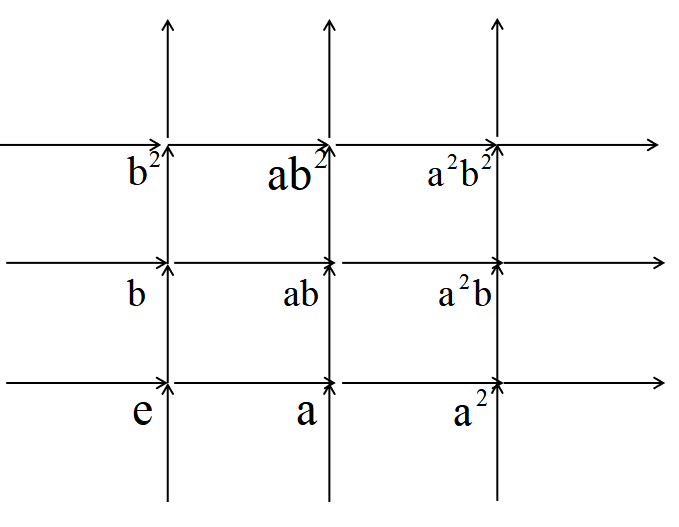
\includegraphics[width=0.3\textwidth]{week11/cayley5.png}}
	\caption{Illustration of Cayley Graph $\langle a,b\mid ab=ba\rangle$}
	\label{Fig:11:7:a}
\end{figure}
\item
The Cayley graph for $G=\langle a,b\rangle$ is shown in Fig.(\ref{Fig:11:7:b}):
\begin{figure}[H]
	\centering{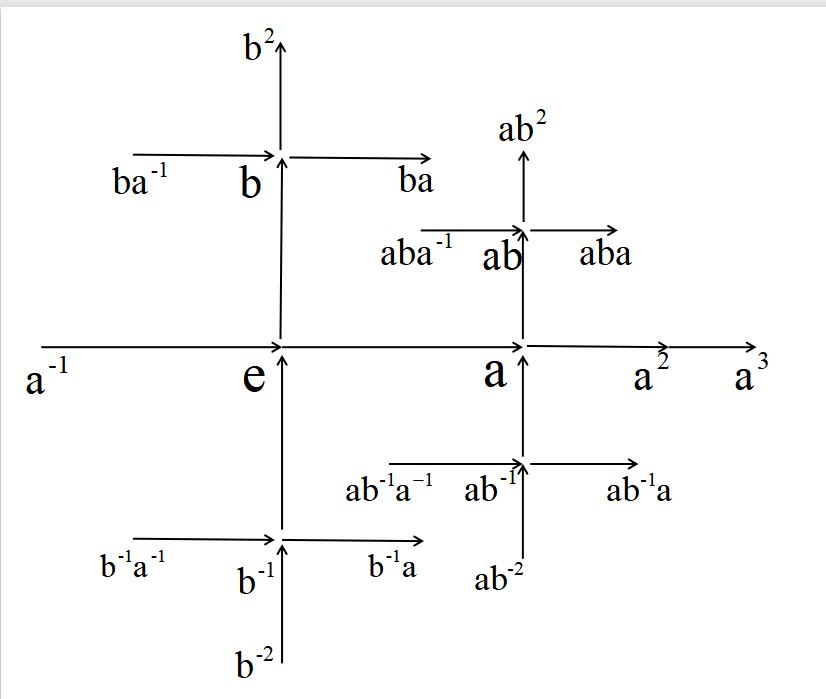
\includegraphics[width=0.3\textwidth]{week11/cayley6.png}}
	\caption{Illustration of Cayley Graph $\langle a,b\mid ab=ba\rangle$}
	\label{Fig:11:7:b}
\end{figure}
\end{enumerate}
\end{example}
\begin{remark}
There could be different presentations $\langle S_1\mid R(S_1)\rangle\cong\langle S_2\mid R(S_2)\rangle$ of the same group.
\end{remark}



\subsection{Fundamental Group}
\paragraph{Motivation}
The fundamental group connects topology and algebra together, by labelling a group to each topological space, which is known as fundamental group.
\paragraph{Why do we need algebra in topology}
Consider the $S^2$ (2-shpere) and $S^1\times S^1$ (torus):
\begin{figure}[H]
	\centering{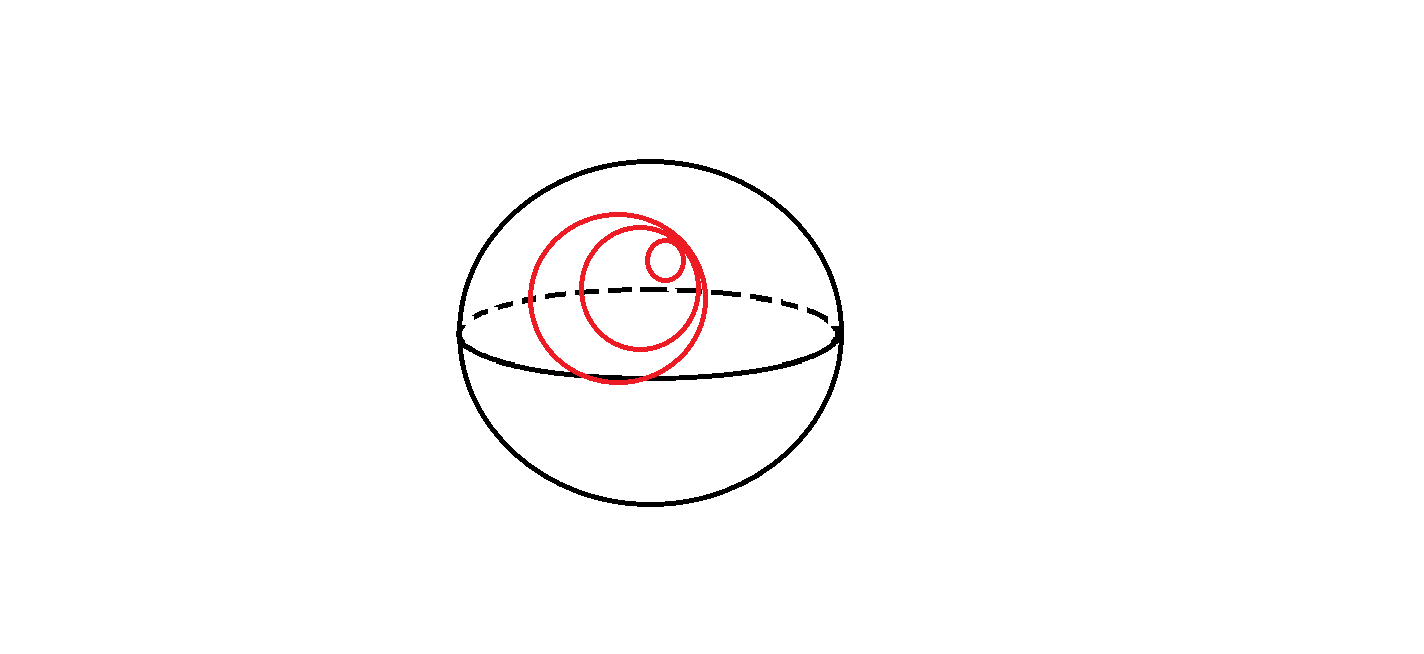
\includegraphics[width=0.5\textwidth]{week11/sphere.png}}
	\caption{Any loop in the sphere can be contracted into a point}
	\label{Fig:11:8:a}
\end{figure}
\begin{figure}[H]
	\centering{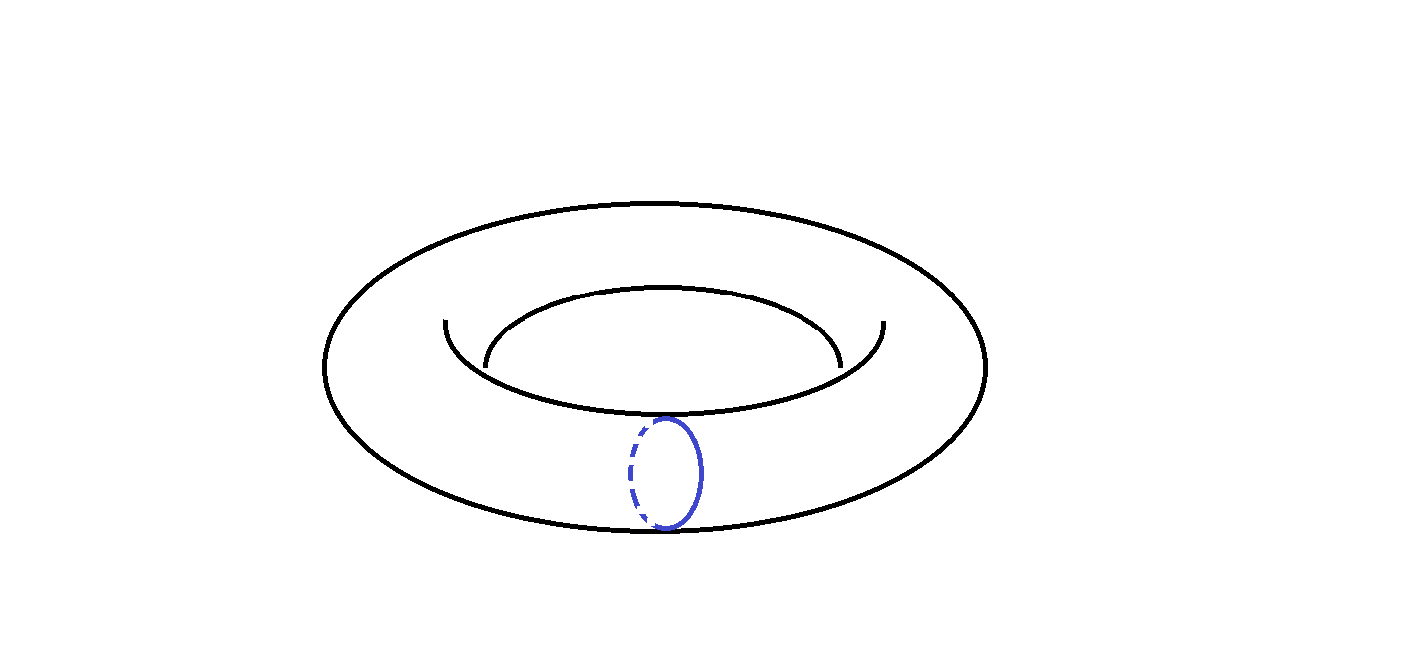
\includegraphics[width=0.5\textwidth]{week11/torus.png}}
	\caption{Some loops in the torus cannot be contracted into a point}
	\label{Fig:11:9:a}
\end{figure}
As can be seen from Fig.(\ref{Fig:11:8:a}) and Fig.(\ref{Fig:11:9:a}), any "loop" on a sphere can be contracted to a point, while some "loop" on a torus cannot. 
We need the algebra to describe this phenomena formally. 

\begin{definition}[loop]
Let $X$ be a topological space.
A \emph{loop} on $X$ is a constant map $\ell:[0,1]\to X$ such that $\ell(0) = \ell(1)$.

We say $\ell$ is based at $b\in X$ if $\ell(0)=\ell(1)=b$.
\end{definition}

\begin{definition}[composite loop]
Suppose that $\bm u,\bm v$ are loops on $X$ based at $b\in X$.
The \emph{composite loop} $u\cdot v$ is given by
\[
u\cdot v=\left\{
\begin{aligned}
u(2t),&\quad\text{if $0\le t\le1/2$}\\
v(2t-1),&\quad\text{if $1/2\le t\le1$}
\end{aligned}
\right.
\]
\end{definition}


\begin{definition}[fundamental group]
The \emph{homotopy class of loops relative to $\{0,1\}$ based at $b\in X$} forms a group.
It is called the \emph{fundamental group} of $X$ based at $b$, denoted as $\pi_1(X,b)$.

More precisely, let 
\[
[\ell]=\{m\mid \text{$m$ is a loop based at $b$ that is homotopic to $\ell$, relative to $\{0,1\}$}\},
\]
and $\pi_1(X,b)=\{[\ell]\mid \text{$\ell$ are loops based at $b$}\}$.
The operation in $\pi_1(X,b)$ is defined as:
\[
[\ell]*[\ell']:=[\ell\cdot\ell'],\quad
\forall [\ell],[\ell']\in\pi_1(X,b).
\]
\end{definition}

\begin{remark}
Two paths $\ell_1,\ell_2:[0,1]\to X$ are homotopic relative to $\{0,1\}$ if we can find $H:[0,1]\times[0,1]\to X$ such that
\[
H(t,0)=\ell_1(t),\quad
H(t,1)=\ell_2(t)
\]
and
\[
H(0,s) = \ell_1(0)=\ell_2(0),\ \forall 0\le s\le1,\quad
H(1,s) = \ell_1(1)=\ell_2(1),\ \forall 0\le s\le 1
\]
\end{remark}

Counter example for homotopy but not relative to $\{0,1\}$: 
\begin{figure}[H]
	\centering
	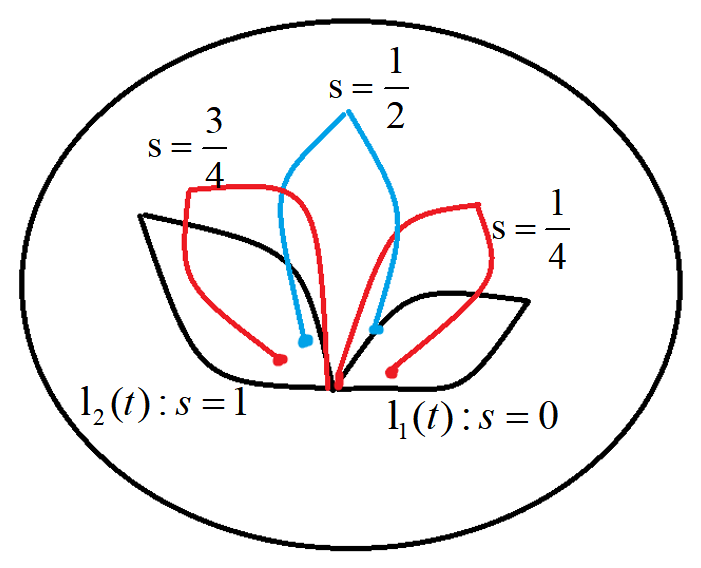
\includegraphics[width=0.4\textwidth]{week11/nonrelative2.png}
	\caption{homotopy not relative to $\{0,1\}$}
	\label{fig: 1:10}
\end{figure}



